%        File: arfc-beamer.tex
%     Created: Sun May 5 10:00 PM 2013 C
%


%\documentclass[11pt,handout]{beamer}
\documentclass[9pt]{beamer}
\usetheme[white]{Illinois}
%\title[short title]{long title}
\title{Full-Core Analysis of Thorium-Fueled Molten Salt Breeder Reactor Using the SERPENT 2 Monte
Carlo Code}
%\subtitle[short subtitle]{long subtitle}
%\subtitle[Short SubTitle]{Mostly Kittens}
%\author[short name]{long name}
\author[Andrei Rykhlevskii]{Andrei Rykhlevskii, Alexander Lindsay, Kathryn Huff\\Advanced Reactors and Fuel Cycles Group}
%\date[short date]{long date}
\date[10.31.2017]{October 31, 2017}
%\institution[short name]{long name}
\institute[UIUC]{University of Illinois at Urbana-Champaign}

%\usepackage{bbding}
\usepackage{tikz}
\usepackage{amsfonts}
\usepackage{amsmath}
\usepackage{caption}  % allows center figures caption
\usepackage{xspace}
\usepackage{notoccite}
\usepackage{graphicx}
\usepackage{subfigure}
\usepackage{booktabs} % nice rules for tables
\usepackage{microtype} % if using PDF
\usepackage{bigints}
\usepackage{minted}
\usepackage{xcolor}
\usepackage{soul}
\newcommand{\hlc}[2][yellow]{{%
    \colorlet{foo}{#1}%
    \sethlcolor{foo}\hl{#2}}%
}
\newcommand{\units}[1] {\:\text{#1}}%
\newcommand{\SN}{S$_N$}%{S$_\text{N}$}%{$S_N$}%
\DeclareMathOperator{\erf}{erf}
%I need some complimentary error funcitons... 
\DeclareMathOperator{\erfc}{erfc}
%page numbers
\setbeamertemplate{footline}[page number]
\setbeamertemplate{caption}[numbered]
%Those icons in the references are terrible looking
\setbeamertemplate{bibliography item}[text]

%%%% Acronym support

\usepackage[acronym,toc]{glossaries}
%\newacronym{<++>}{<++>}{<++>}
\newacronym[longplural={metric tons of heavy metal}]{MTHM}{MTHM}{metric ton of heavy metal}
\newacronym{ABM}{ABM}{agent-based modeling}
\newacronym{ACDIS}{ACDIS}{Program in Arms Control \& Domestic and International Security}
\newacronym{AHTR}{AHTR}{Advanced High Temperature Reactor}
\newacronym{ANDRA}{ANDRA}{Agence Nationale pour la gestion des D\'echets RAdioactifs, the French National Agency for Radioactive Waste Management}
\newacronym{ANL}{ANL}{Argonne National Laboratory}
\newacronym{ANS}{ANS}{American Nuclear Society}
\newacronym{API}{API}{application programming interface}
\newacronym{ARE}{ARE}{Aircraft Reactor Experiment}
\newacronym{ARFC}{ARFC}{Advanced Reactors and Fuel Cycles}
\newacronym{ASME}{ASME}{American Society of Mechanical Engineers}
\newacronym{ATWS}{ATWS}{Anticipated Transient Without Scram}
\newacronym{BDBE}{BDBE}{Beyond Design Basis Event}
\newacronym{BIDS}{BIDS}{Berkeley Institute for Data Science}
\newacronym{CAFCA}{CAFCA}{ Code for Advanced Fuel Cycles Assessment }
\newacronym{CDTN}{CDTN}{Centro de Desenvolvimento da Tecnologia Nuclear}
\newacronym{CEA}{CEA}{Commissariat \`a l'\'Energie Atomique et aux \'Energies Alternatives}
\newacronym{CI}{CI}{continuous integration}
\newacronym{CNEN}{CNEN}{Comiss\~{a}o Nacional de Energia Nuclear}
\newacronym{CNERG}{CNERG}{Computational Nuclear Engineering Research Group}
\newacronym{COSI}{COSI}{Commelini-Sicard}
\newacronym{COTS}{COTS}{commercial, off-the-shelf}
\newacronym{CSNF}{CSNF}{commercial spent nuclear fuel}
\newacronym{CTAH}{CTAHs}{Coiled Tube Air Heaters}
\newacronym{CUBIT}{CUBIT}{CUBIT Geometry and Mesh Generation Toolkit}
\newacronym{CURIE}{CURIE}{Centralized Used Fuel Resource for Information Exchange}
\newacronym{DAG}{DAG}{directed acyclic graph}
\newacronym{DANESS}{DANESS}{Dynamic Analysis of Nuclear Energy System Strategies}
\newacronym{DBE}{DBE}{Design Basis Event}
\newacronym{DESAE}{DESAE}{Dynamic Analysis of Nuclear Energy Systems Strategies}
\newacronym{DHS}{DHS}{Department of Homeland Security}
\newacronym{DOE}{DOE}{Department of Energy}
\newacronym{DRACS}{DRACS}{Direct Reactor Auxiliary Cooling System}
\newacronym{DRE}{DRE}{dynamic resource exchange}
\newacronym{DSNF}{DSNF}{DOE spent nuclear fuel}
\newacronym{DYMOND}{DYMOND}{Dynamic Model of Nuclear Development }
\newacronym{EBS}{EBS}{Engineered Barrier System}
\newacronym{EDF}{EDF}{Électricité de France}
\newacronym{EDZ}{EDZ}{Excavation Disturbed Zone}
\newacronym{EIA}{EIA}{U.S. Energy Information Administration}
\newacronym{EPA}{EPA}{Environmental Protection Agency}
\newacronym{EPR}{EPR}{European Pressurized Reactors}
\newacronym{EP}{EP}{Engineering Physics}
\newacronym{EU}{EU}{European Union}
\newacronym{FCO}{FCO}{Fuel Cycle Options}
\newacronym{FCT}{FCT}{Fuel Cycle Technology}
\newacronym{FEHM}{FEHM}{Finite Element Heat and Mass Transfer}
\newacronym{FEPs}{FEPs}{Features, Events, and Processes}
\newacronym{FHR}{FHR}{Fluoride-Salt-Cooled High-Temperature Reactor}
\newacronym{FLiBe}{FLiBe}{Fluoride-Lithium-Beryllium}
\newacronym{FP}{FP}{Fission Products}
\newacronym{GDSE}{GDSE}{Generic Disposal System Environment}
\newacronym{GDSM}{GDSM}{Generic Disposal System Model}
\newacronym{GENIUSv1}{GENIUSv1}{Global Evaluation of Nuclear Infrastructure Utilization Scenarios, Version 1}
\newacronym{GENIUSv2}{GENIUSv2}{Global Evaluation of Nuclear Infrastructure Utilization Scenarios, Version 2}
\newacronym{GENIUS}{GENIUS}{Global Evaluation of Nuclear Infrastructure Utilization Scenarios}
\newacronym{GPAM}{GPAM}{Generic Performance Assessment Model}
\newacronym{GRSAC}{GRSAC}{Graphite Reactor Severe Accident Code}
\newacronym{GUI}{GUI}{graphical user interface}
\newacronym{HLW}{HLW}{high level waste}
\newacronym{HPC}{HPC}{high-performance computing}
\newacronym{HTC}{HTC}{high-throughput computing}
\newacronym{HTGR}{HTGR}{High Temperature Gas-Cooled Reactor}
\newacronym{IAEA}{IAEA}{International Atomic Energy Agency}
\newacronym{IEMA}{IEMA}{Illinois Emergency Mangament Agency}
\newacronym{IHLRWM}{IHLRWM}{International High Level Radioactive Waste Management}
\newacronym{INL}{INL}{Idaho National Laboratory}
\newacronym{IPRR1}{IRP-R1}{Instituto de Pesquisas Radioativas Reator 1}
\newacronym{IRP}{IRP}{Integrated Research Project}
\newacronym{ISFSI}{ISFSI}{Independent Spent Fuel Storage Installation}
\newacronym{ISRG}{ISRG}{Independent Student Research Group}
\newacronym{JFNK}{JFNK}{Jacobian-Free Newton Krylov}
\newacronym{LANL}{LANL}{Los Alamos National Laboratory}
\newacronym{LBNL}{LBNL}{Lawrence Berkeley National Laboratory}
\newacronym{LCOE}{LCOE}{levelized cost of electricity}
\newacronym{LDRD}{LDRD}{laboratory directed research and development}
\newacronym{LFR}{LFR}{Lead-Cooled Fast Reactor}
\newacronym{LLNL}{LLNL}{Lawrence Livermore National Laboratory}
\newacronym{LMFBR}{LMFBR}{Liquid Metal Fast Breeder Reactor}
\newacronym{LOFC}{LOFC}{Loss of Forced Cooling}
\newacronym{LOHS}{LOHS}{Loss of Heat Sink}
\newacronym{LOLA}{LOLA}{Loss of Large Area}
\newacronym{LP}{LP}{linear program}
\newacronym{LWR}{LWR}{Light Water Reactor}
\newacronym{MAGNOX}{MAGNOX}{Magnesium Alloy Graphie Moderated Gas Cooled Uranium Oxide Reactor}
\newacronym{MA}{MA}{minor actinide}
\newacronym{MCNP}{MCNP}{Monte Carlo N-Particle code}
\newacronym{MILP}{MILP}{mixed-integer linear program}
\newacronym{MIT}{MIT}{the Massachusetts Institute of Technology}
\newacronym{MOAB}{MOAB}{Mesh-Oriented datABase}
\newacronym{MOOSE}{MOOSE}{Multiphysics Object-Oriented Simulation Environment}
\newacronym{MOX}{MOX}{mixed oxide}
\newacronym{MSBR}{MSBR}{Molten Salt Breeder Reactor}
\newacronym{MSRE}{MSRE}{Molten Salt Reactor Experiment}
\newacronym{MSR}{MSR}{Molten Salt Reactor}
\newacronym{NAGRA}{NAGRA}{National Cooperative for the Disposal of Radioactive Waste}
\newacronym{NEAMS}{NEAMS}{Nuclear Engineering Advanced Modeling and Simulation}
\newacronym{NEUP}{NEUP}{Nuclear Energy University Programs}
\newacronym{NFCSim}{NFCSim}{Nuclear Fuel Cycle Simulator}
\newacronym{NGNP}{NGNP}{Next Generation Nuclear Plant}
\newacronym{NMWPC}{NMWPC}{Nuclear MW Per Capita}
\newacronym{NNSA}{NNSA}{National Nuclear Security Administration}
\newacronym{NPP}{NPP}{Nuclear Power Plant}
\newacronym{NPRE}{NPRE}{Department of Nuclear, Plasma, and Radiological Engineering}
\newacronym{NQA1}{NQA-1}{Nuclear Quality Assurance - 1}
\newacronym{NRC}{NRC}{Nuclear Regulatory Commission}
\newacronym{NSF}{NSF}{National Science Foundation}
\newacronym{NSSC}{NSSC}{Nuclear Science and Security Consortium}
\newacronym{NUWASTE}{NUWASTE}{Nuclear Waste Assessment System for Technical Evaluation}
\newacronym{NWF}{NWF}{Nuclear Waste Fund}
\newacronym{NWTRB}{NWTRB}{Nuclear Waste Technical Review Board}
\newacronym{OCRWM}{OCRWM}{Office of Civilian Radioactive Waste Management}
\newacronym{ORION}{ORION}{ORION}
\newacronym{ORNL}{ORNL}{Oak Ridge National Laboratory}
\newacronym{PARCS}{PARCS}{Purdue Advanced Reactor Core Simulator}
\newacronym{PBAHTR}{PB-AHTR}{Pebble Bed Advanced High Temperature Reactor}
\newacronym{PBFHR}{PB-FHR}{Pebble-Bed Fluoride-Salt-Cooled High-Temperature Reactor}
\newacronym{PEI}{PEI}{Peak Environmental Impact}
\newacronym{PH}{PRONGHORN}{PRONGHORN}
\newacronym{PRIS}{PRIS}{Power Reactor Information System}
\newacronym{PRKE}{PRKE}{Point Reactor Kinetics Equations}
\newacronym{PSPG}{PSPG}{Pressure-Stabilizing/Petrov-Galerkin}
\newacronym{PWAR}{PWAR}{Pratt and Whitney Aircraft Reactor}
\newacronym{PWR}{PWR}{Pressurized Water Reactor}
\newacronym{PyNE}{PyNE}{Python toolkit for Nuclear Engineering}
\newacronym{PyRK}{PyRK}{Python for Reactor Kinetics}
\newacronym{QA}{QA}{quality assurance}
\newacronym{RDD}{RD\&D}{Research Development and Demonstration}
\newacronym{RD}{R\&D}{Research and Development}
\newacronym{RELAP}{RELAP}{Reactor Excursion and Leak Analysis Program}
\newacronym{RIA}{RIA}{Reactivity Insertion Accident}
\newacronym{RIF}{RIF}{Region-Institution-Facility}
\newacronym{SFR}{SFR}{Sodium-Cooled Fast Reactor}
\newacronym{SINDAG}{SINDA{\textbackslash}G}{Systems Improved Numerical Differencing Analyzer $\backslash$ Gaski}
\newacronym{SKB}{SKB}{Svensk K\"{a}rnbr\"{a}nslehantering AB}
\newacronym{SNF}{SNF}{spent nuclear fuel}
\newacronym{SNL}{SNL}{Sandia National Laboratory}
\newacronym{STC}{STC}{specific temperature change}
\newacronym{SUPG}{SUPG}{Streamline-Upwind/Petrov-Galerkin}
\newacronym{SWF}{SWF}{Separations and Waste Forms}
\newacronym{SWU}{SWU}{Separative Work Unit}
\newacronym{TRIGA}{TRIGA}{Training Research Isotope General Atomic}
\newacronym{TRISO}{TRISO}{Tristructural Isotropic}
\newacronym{TSM}{TSM}{Total System Model}
\newacronym{TSPA}{TSPA}{Total System Performance Assessment for the Yucca Mountain License Application}
\newacronym{ThOX}{ThOX}{thorium oxide}
\newacronym{UFD}{UFD}{Used Fuel Disposition}
\newacronym{UML}{UML}{Unified Modeling Language}
\newacronym{UOX}{UOX}{uranium oxide}
\newacronym{UQ}{UQ}{uncertainty quantification}
\newacronym{US}{US}{United States}
\newacronym{UW}{UW}{University of Wisconsin}
\newacronym{VISION}{VISION}{the Verifiable Fuel Cycle Simulation Model}
\newacronym{VVER}{VVER}{Voda-Vodyanoi Energetichesky Reaktor (Russian Pressurized Water Reactor)}
\newacronym{VV}{V\&V}{verification and validation}
\newacronym{WIPP}{WIPP}{Waste Isolation Pilot Plant}
\newacronym{YMR}{YMR}{Yucca Mountain Repository Site}


\makeglossaries

%try to get rid of header on title page\dots
\makeatletter
    \newenvironment{withoutheadline}{
        \setbeamertemplate{headline}[default]
        \def\beamer@entrycode{\vspace*{-\headheight}}
    }{}
\makeatother

\begin{document}
%%%%%%%%%%%%%%%%%%%%%%%%%%%%%%%%%%%%%%%%%%%%%%%%%%%%%%%%%%%%%
%% From uw-beamer Here's a handy bit of code to place at 
%% the beginning of your presentation (after \begin{document}):
\newcommand*{\alphabet}{ABCDEFGHIJKLMNOPQRSTUVWXYZabcdefghijklmnopqrstuvwxyz}
\newlength{\highlightheight}
\newlength{\highlightdepth}
\newlength{\highlightmargin}
\setlength{\highlightmargin}{2pt}
\settoheight{\highlightheight}{\alphabet}
\settodepth{\highlightdepth}{\alphabet}
\addtolength{\highlightheight}{\highlightmargin}
\addtolength{\highlightdepth}{\highlightmargin}
\addtolength{\highlightheight}{\highlightdepth}
\newcommand*{\Highlight}{\rlap{\textcolor{HighlightBackground}{\rule[-\highlightdepth]{\linewidth}{\highlightheight}}}}
%%%%%%%%%%%%%%%%%%%%%%%%%%%%%%%%%%%%%%%%%%%%%%%%%%%%%%%%%%%%%
%%--------------------------------%%
\begin{withoutheadline}
\frame{
  \titlepage
}
\end{withoutheadline}

%%--------------------------------%%
\AtBeginSection[]{
\begin{frame}
  \frametitle{Outline}
  \tableofcontents[currentsection]
\end{frame}
}

\section{Background}
\subsection{Motivation}

\begin{frame}
  \frametitle{Reactor systems potentially meeting the Generation IV goals}
               \begin{figure}[t]
                \vspace*{-0.1in}
                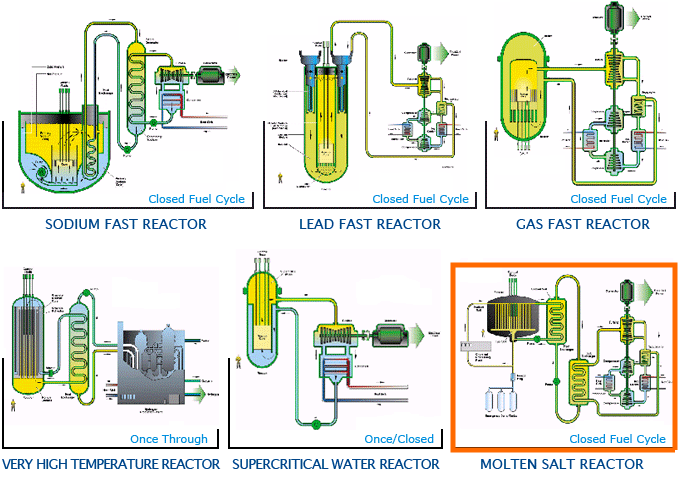
\includegraphics[height=0.65\textwidth]{./images/6_types.png}
                 \caption{Potential Generation IV reactors \cite{ABRAM2008}.}
               \end{figure}
              
\end{frame}

\begin{frame}
  \frametitle{Why Molten Salt Reactors?}
                  \vspace*{-0.1in}
              \begin{block}{Main advantages of liquid-fueled \glspl{MSR}\cite{elsheikh_safety_2013}}
               \begin{enumerate}
                \item High average coolant temperature (600-750$^{\circ}$C) $\Rightarrow$ high thermal efficiency.
                \item May operate with epithermal or fast neutron spectrums.
                \item Various fuels can be used ($^{235}$U, $^{233}$U, Thorium, U/Pu).
                \item Liquid fuel has strong negative temperature feedback.
                \item Liquid fuel drains into tanks in emergency.
                \item High fuel utilization $\Rightarrow$ less nuclear waste generated.
                \item Online reprocessing and refueling.
               \end{enumerate}
               \end{block}
                  \vspace*{-0.1in}               
               \begin{block}{Main advantages of \gls{MSBR}\cite{robertson_conceptual_1971}}
               \begin{enumerate}
                \item Breed fissile $^{233}$U from $^{232}$Th (breeding ratio 1.06).
                \item $^{233}$U, $^{235}$U, or $^{239}$Pu for the initial fissile loading.
                \item Thorium cycle limits plutonium and minor actinides.
                \item Could transmute \gls{LWR} spent fuel.
               \end{enumerate}
               \end{block}

\end{frame}

\begin{frame}
  \frametitle{Molten Salt Reactor Experiment vs Molten Salt Breeder Reactor}
  \begin{columns}
    \column[t]{5.6cm}
               \begin{figure}[t]
                \vspace*{-0.3in}
                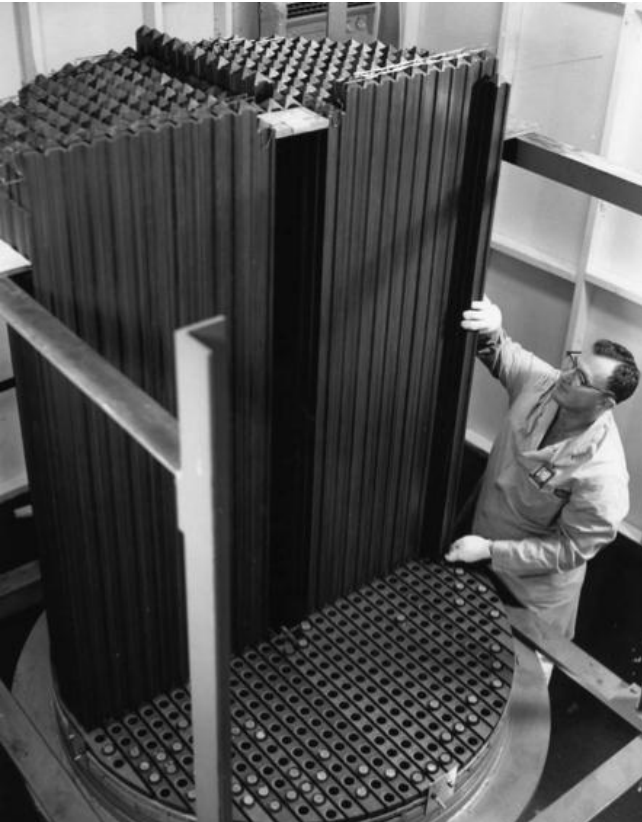
\includegraphics[height=0.7\textwidth]{./images/msre_view.png}
                \vspace*{-0.2in}
      \end{figure}
     \begin{block}{\gls{MSRE}}
       \begin{enumerate}
              \item 8 MW$_{th}$
               \item Fuel salt
                \begin{itemize}
                   \item $^7$LiF-BeF$_2$-ZrF$_4$-UF$_4$
                   \item $^7$LiF-BeF$_2$-ZrF$_4$-UF$_4$-PuF$_3$
                \end{itemize}  
              \item First use of $^{233}$U and mixed U/Pu
              \item Single region core
              \item Operated: 1965-1969 at ORNL
              \end{enumerate}
     \end{block}
     \column[t]{5.6cm}
           \begin{figure}[t]
                \vspace*{-0.3in}
                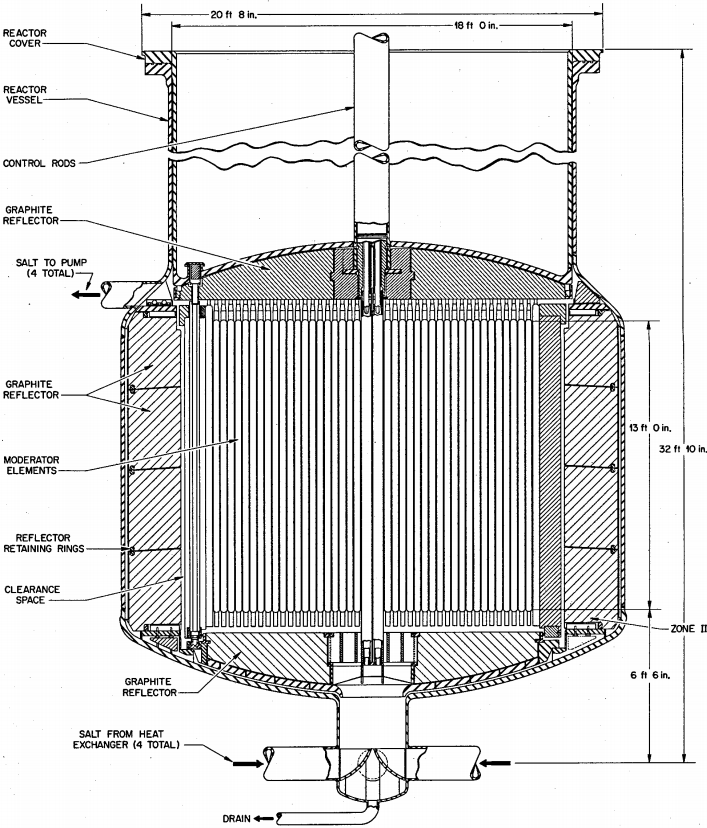
\includegraphics[height=0.7\textwidth]{./images/msbr_plain.png}
                \vspace*{-0.2in}
      \end{figure}
   \begin{block}{\glsfirst{MSBR} \cite{robertson_conceptual_1971}}
       \begin{enumerate}
       \item 2.25GW$_{th}$, 1GW$_e$
       \item Fuel salt
         \begin{itemize}
         \item $^7$LiF-BeF$_2$-ThF$_4$-$^{233}$UF$_4$
         \item $^7$LiF-BeF$_2$-ThF$_4$-$^{233}$UF$_4$-$^{239}$PuF$_3$
         \end{itemize}  
       \item Breeding ratio 1.06
       \item Single fluid/two-region core design
       \item Chemical salt processing plant
      \end{enumerate}
     \end{block}
  \end{columns}
              
 \end{frame}

\subsection{Objectives}
\begin{frame}
  \frametitle{Research objectives}
                  \vspace*{-0.1in}
              \begin{block}{Goals of current study}
               \begin{enumerate}
                \item Develop simplified single-cell \gls{MSBR} model using the continuous-energy SERPENT 2 Monte Carlo reactor
					physics software \cite{leppanen_serpent_2012}.
                \item Using the built-in SERPENT 2 depletion  capabilities simulate online reprocessing and refueling regime.
                \item Find the equilibrium core composition for the \gls{MSBR}.
               \end{enumerate}
               \end{block}
               
               \begin{block}{What is next?}
               \begin{enumerate}
                \item Depletion simulation using a full-core, 3-D, high-fidelity \gls{MSBR} model.
                \item Additional SERPENT 2 flow control system will evaluate material flows.
                \item Optimization of reprocessing parameters and reactor design.
                \item Determine and compare major safety characteristics for initial and equilibrium fuel composition.
               \end{enumerate}
               \end{block}

\end{frame}



\section{Geometry}
\begin{frame}
  \frametitle{Geometry of \gls{MSBR} model for SERPENT 2}
    \vspace{-0.2in}
      \begin{figure}[t]
    \hspace*{-0.35in}
        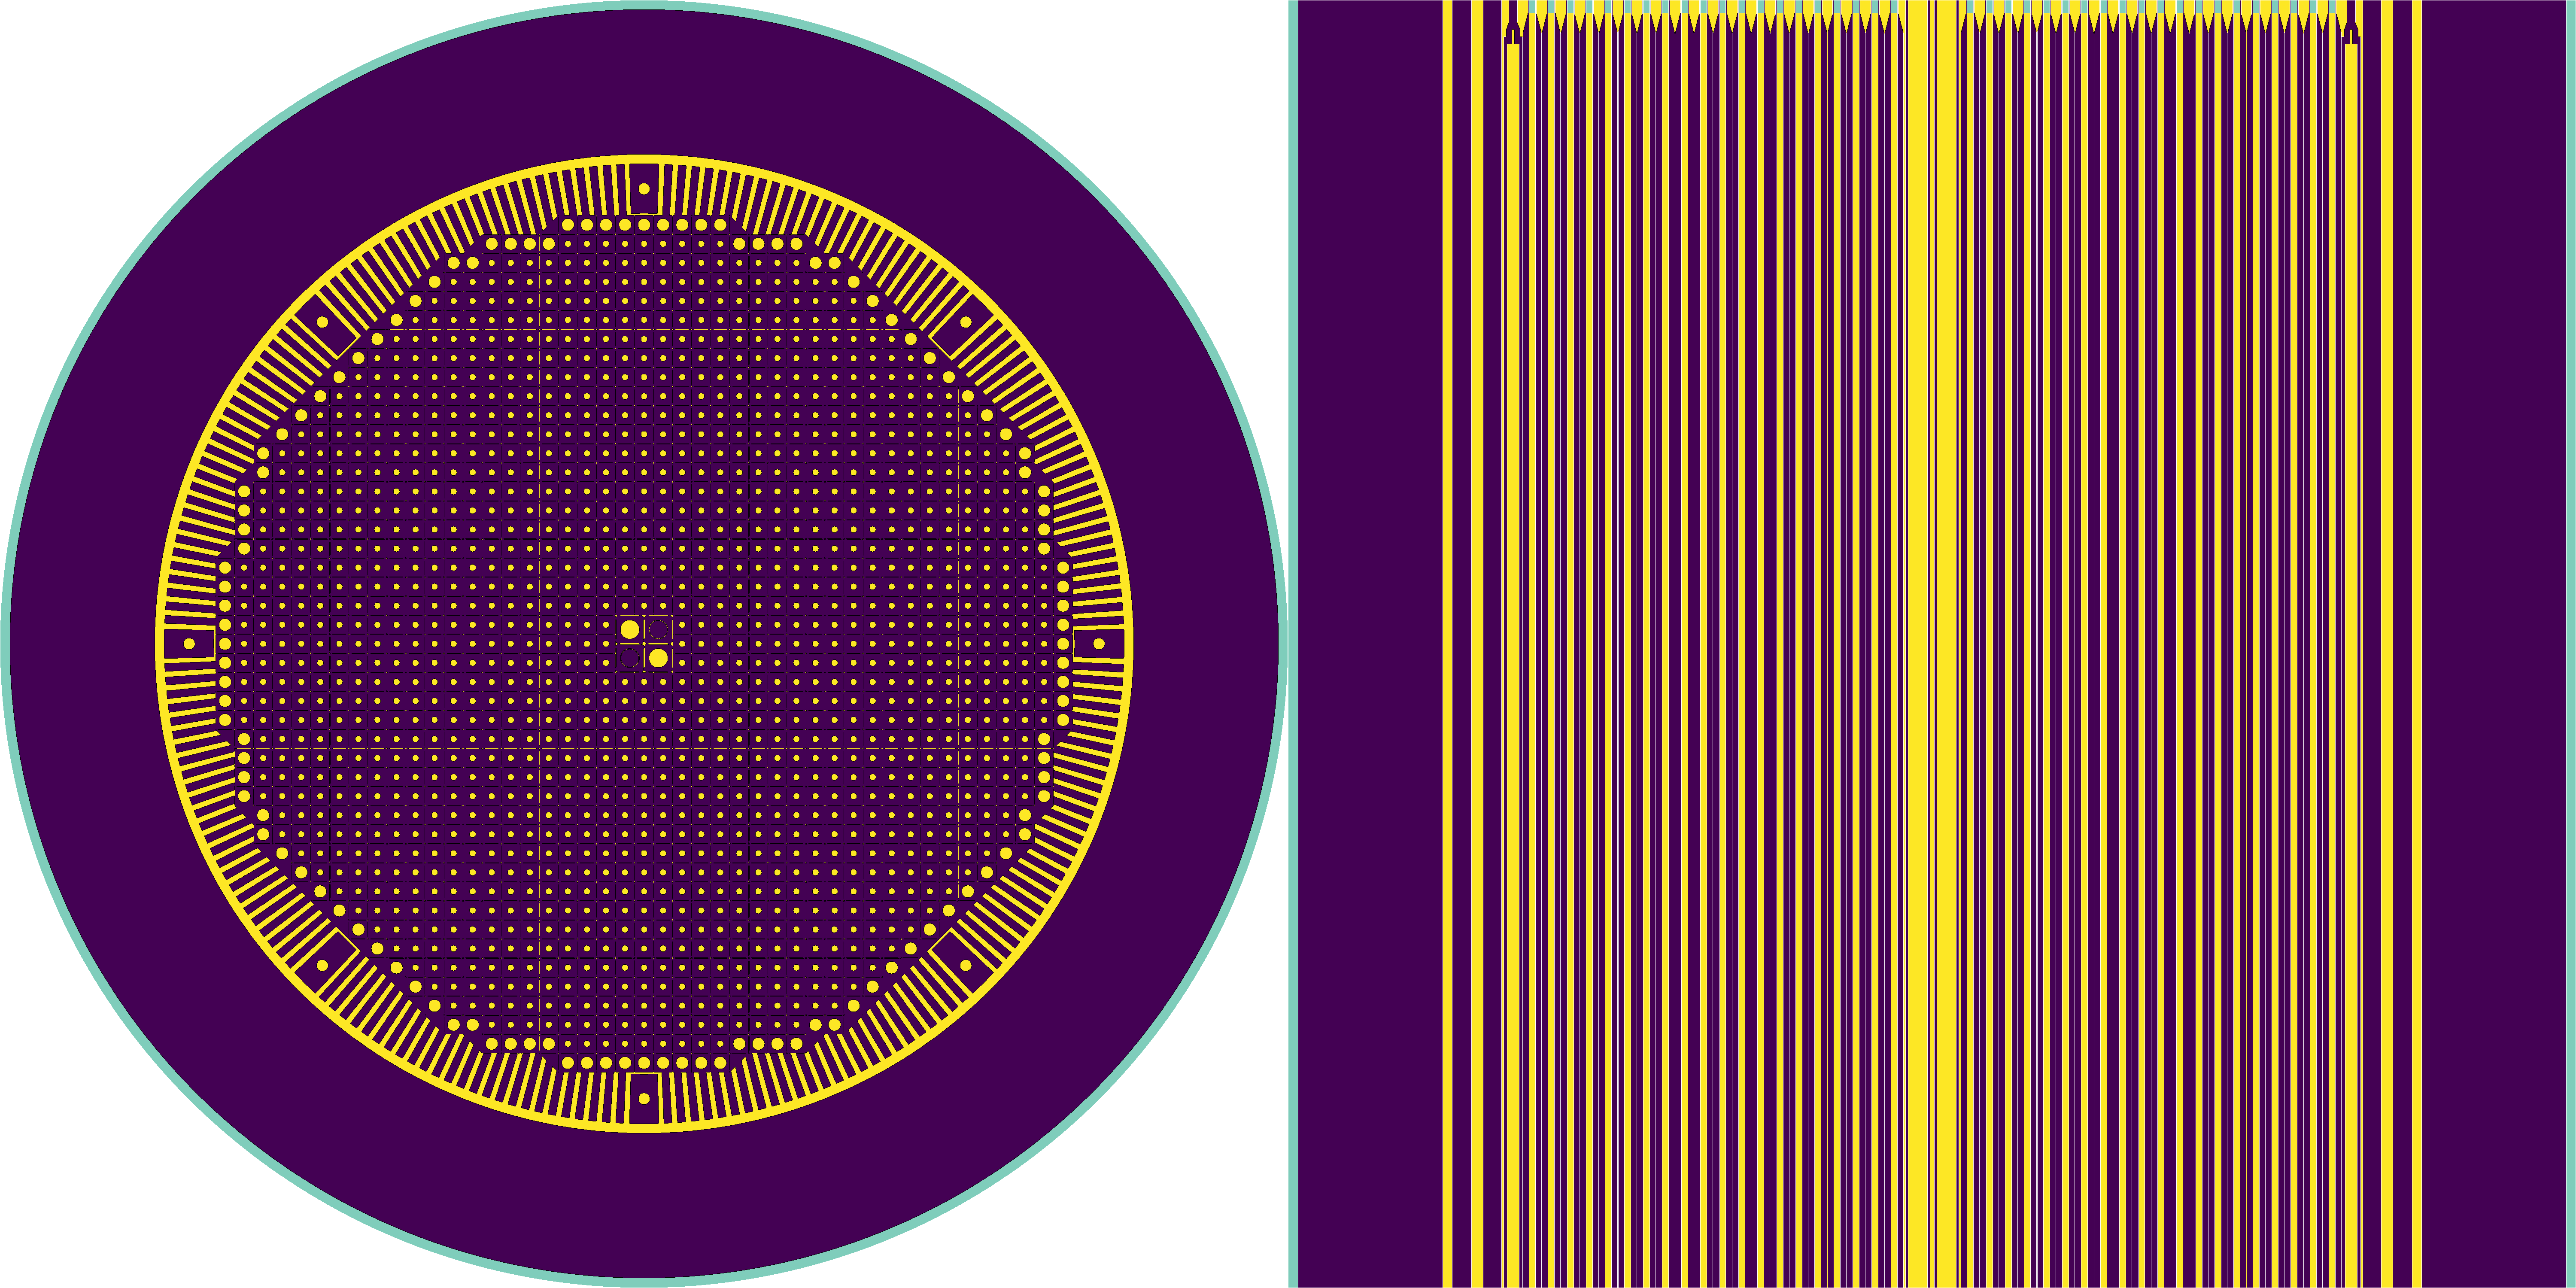
\includegraphics[height=0.75\textheight]{./images/geometry_main_views.png}
        \caption{Plan (left) and elevation (right) view of \gls{MSBR} model}
  \end{figure}


\end{frame}

\begin{frame}
  \frametitle{Graphite elements geometry}
  \begin{figure}[t]
     \vspace{-0.20in}
       \hspace*{-0.4in}
       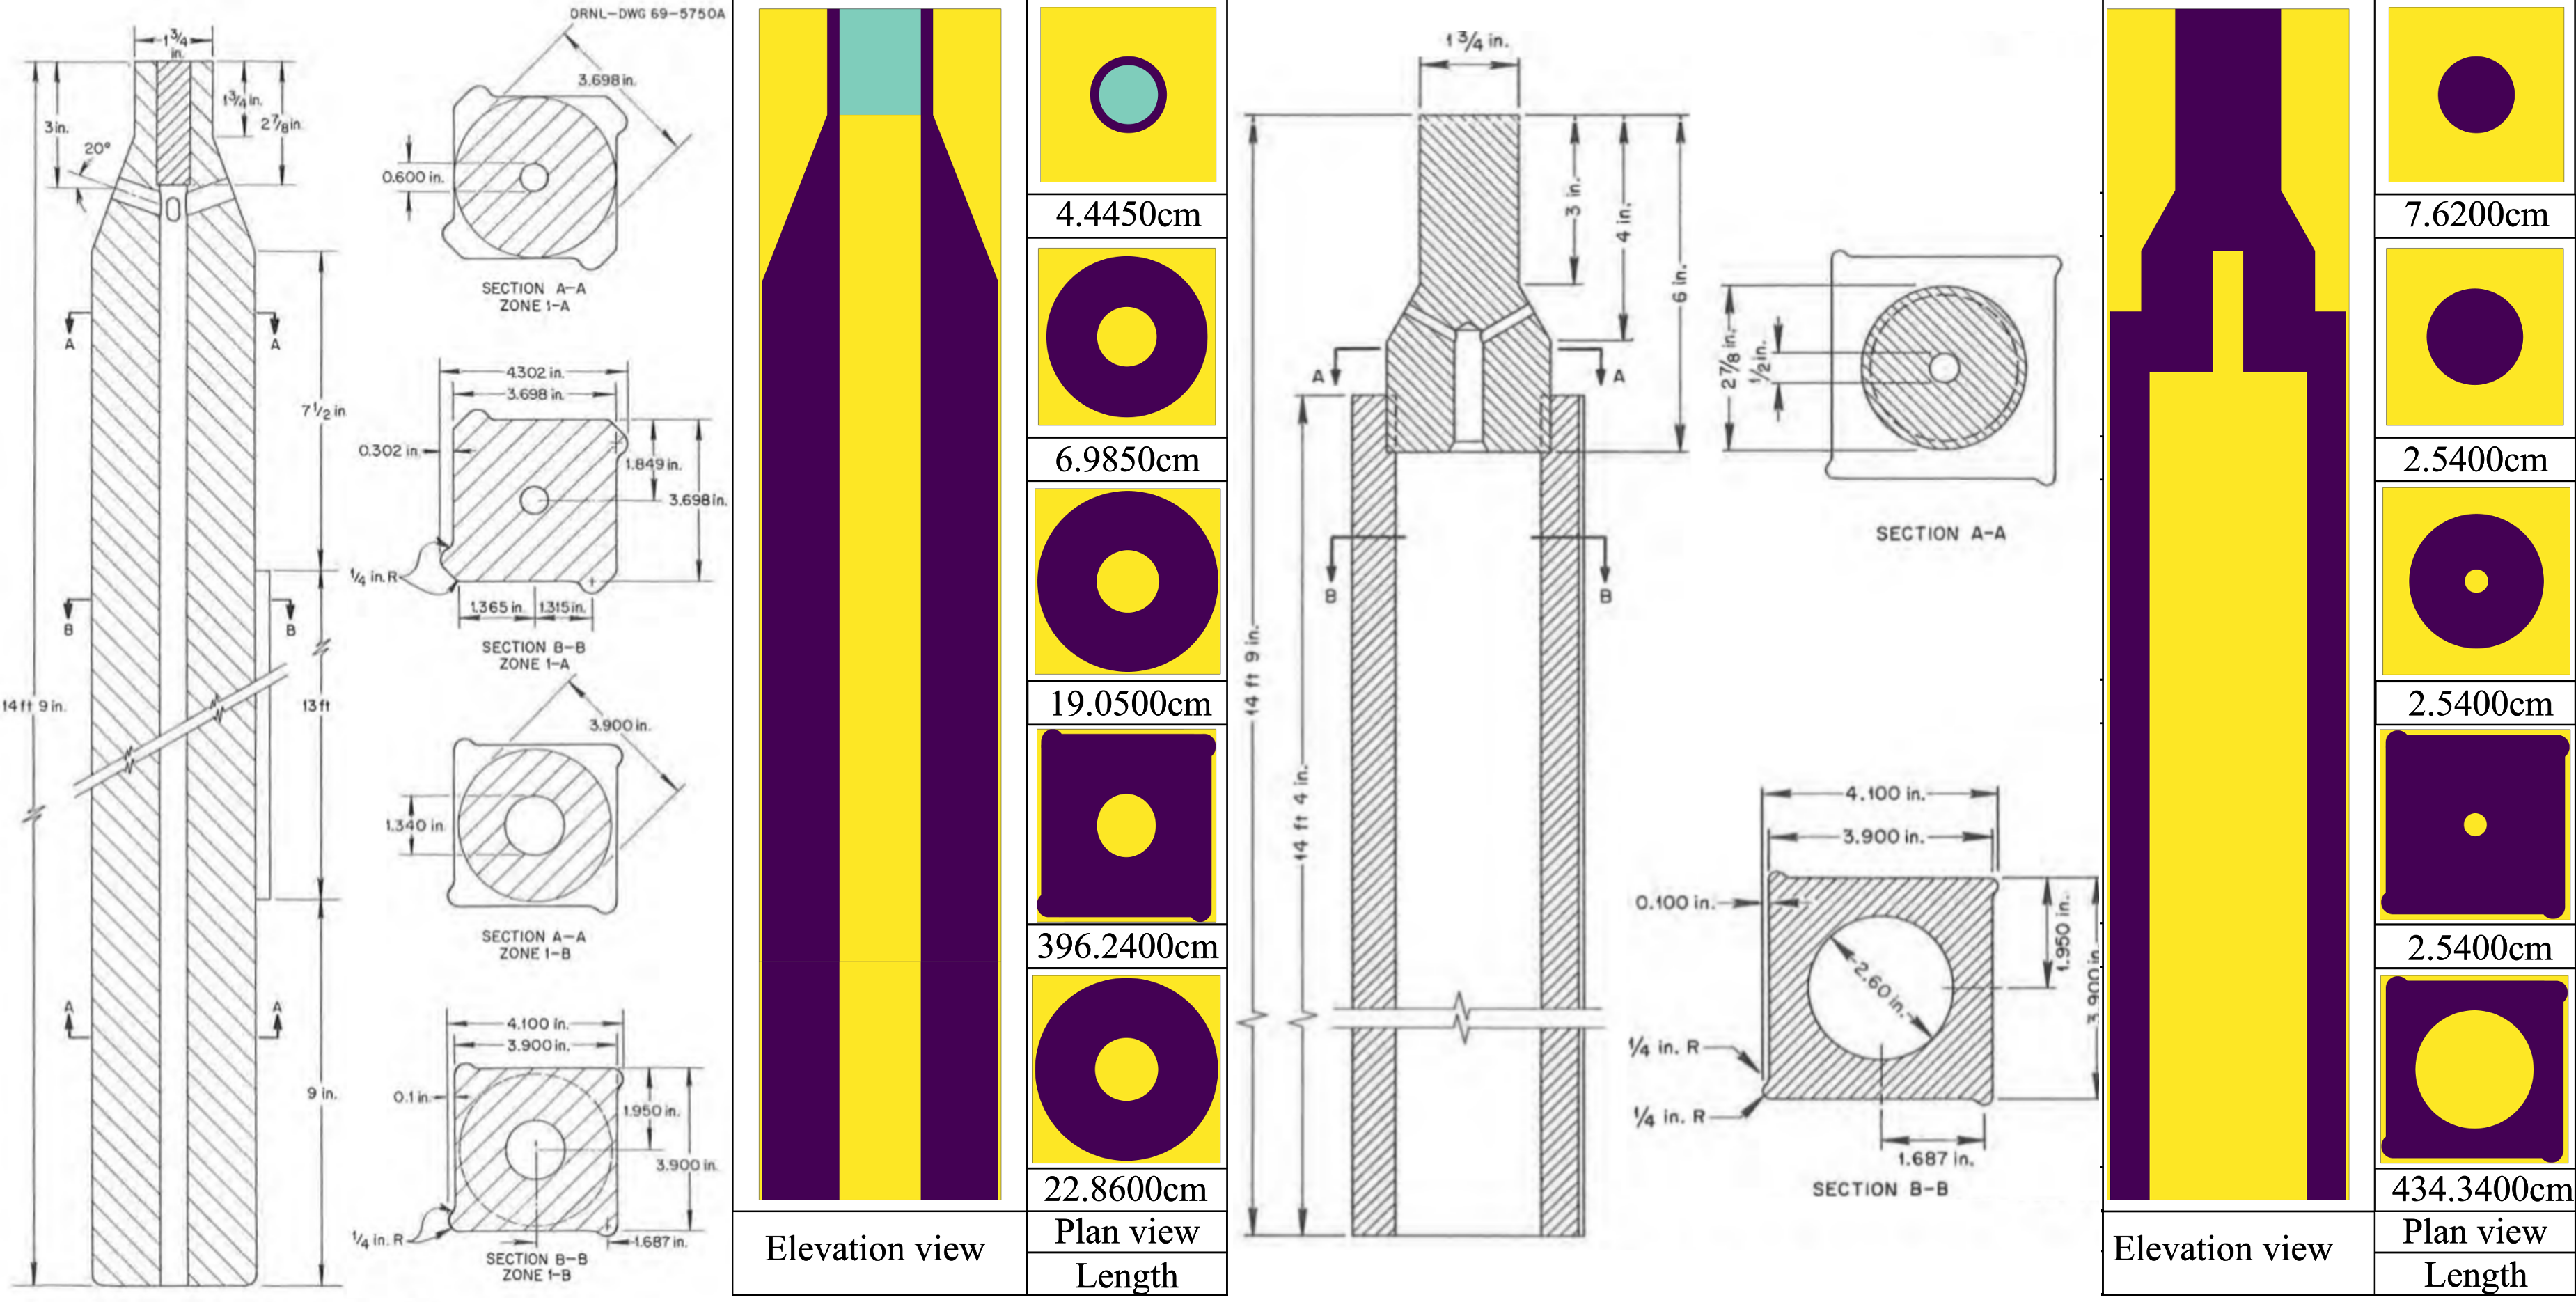
\includegraphics[height=0.77\textheight]{./images/zone_I_element.png}
            \vspace{-0.05in}
            \caption{Zone I (left) and Zone II (right) reference design
              \cite{robertson_conceptual_1971} and model.}
  \end{figure}
  
           \vspace{-0.1in}
      Volume fraction of fuel salt in zones I and II was 0.132 and 0.37 respectively.
     
\end{frame}

\begin{frame}
  \frametitle{Core Zone II}
  \begin{figure}[t]
     \vspace{-0.25in}
       \hspace*{-0.43in}
       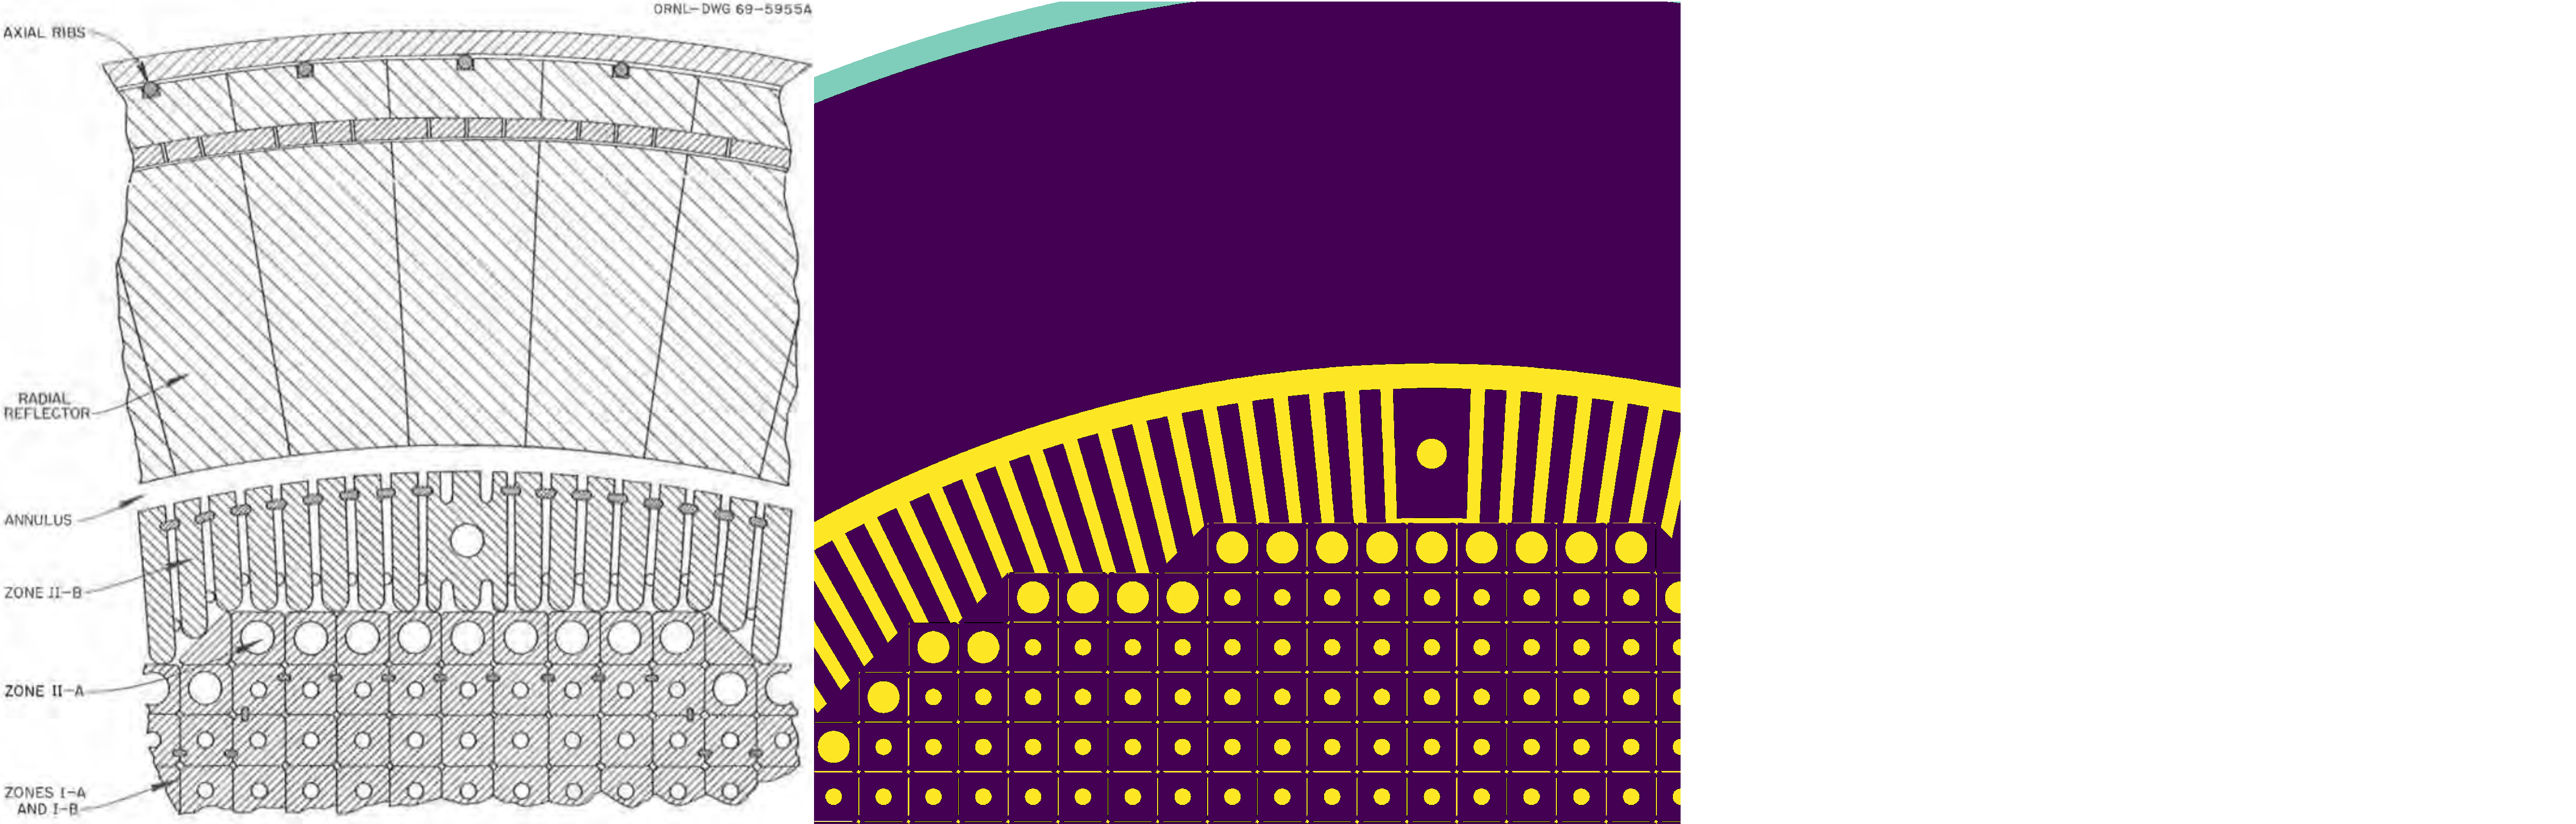
\includegraphics[height=0.77\textheight]{./images/reflector_and_elements.png}
            \caption{Detailed plan view of graphite reflector and moderator elements.}
  \end{figure}
           \vspace{-0.1in}
\end{frame}

\begin{frame}
  \frametitle{Approximations and assumptions}
              \begin{block}{Geometry simplifications}
               \begin{enumerate}
               \item Zone II-B elements simplified into right-circular
                 cylindrical shapes with central channels.
               \item Axial ribs in Zone I outer layer, Zone II-B and reflector was not
                 described in the model.
               \end{enumerate}
               \end{block}

               \begin{block}{Simulation conditions and nuclear data}
               \begin{enumerate}
               \item Two graphite control rods are fully inserted.
               \item Two safety rods are fully withdrawn.
               \item Moderator and fuel temperature is 900K.
               \item $10^5$ neutrons per cycle for a total of 1000 cycles,
                 the first 50 are inactive.
               \item ENDF/B-VII cross sections were used.
               \end{enumerate}
               \end{block}
\end{frame}


\section{Results and discussion}
\begin{frame}
  \frametitle{Infinite multiplication factor for unit cell model}
    \begin{columns}
    \column[t]{7cm}
   \vspace{-0.35in}
  \begin{figure}[t]
   \hspace*{-0.2in}
   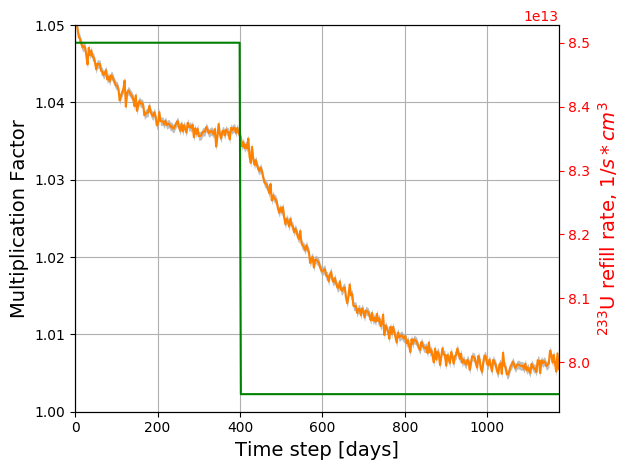
\includegraphics[height=0.75\textheight]{./images/keff.png}
   \vspace{-0.05in}
   \caption{Infinite multiplication factor during a 1200 days depletion simulation. The confidence interval $\pm\sigma$ is shaded.}
    \end{figure}

    \column[t]{4.5cm}
       \begin{itemize}
        \item Strong absorbers ($^{233}$Th,$^{234}$U) accumulating in the begining of cycle. 
   		\item Fissile materials other than $^{233}$U producing in the core ($^{235}$U, $^{239}$Pu).
   		\item Fresh fuel refill rate was changed after 400 days of operation to adjust this effects.
   		\item The multiplication factor stabilizes after approximately 950 days.
       \end{itemize}
     \end{columns}
\end{frame}

\begin{frame}
  \frametitle{Fuel salt composition evolution}
    \begin{columns}
    \column[t]{7cm}
   \vspace{-0.35in}
  \begin{figure}[t]
   \hspace*{-0.15in}
   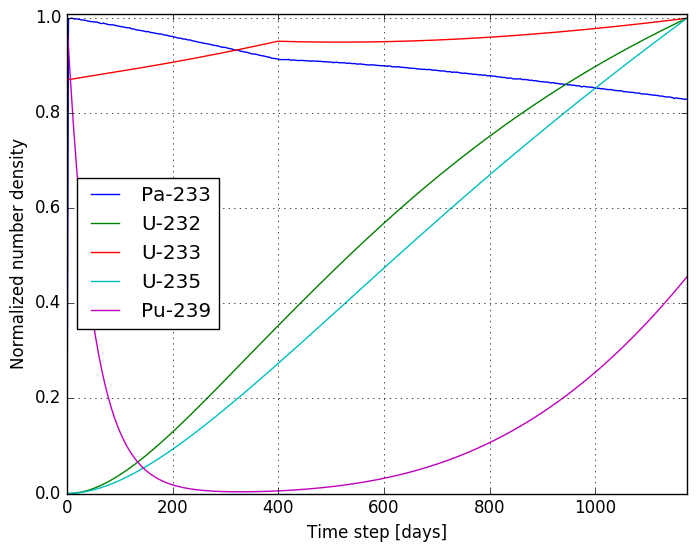
\includegraphics[height=0.75\textheight]{./images/fuel_composition.png}
   \vspace{-0.05in}
   \caption{Normalized number density of major isotopes during 1200 days of depletion.}
    \end{figure}

    \column[t]{5cm}
       \begin{itemize}
        \item Number density of $^{233}$Pa is negligible (10$^{16}$ 1/cm$^3$) but some small amount of it is produced
during the 3-day reprocessing period. 
   		\item Fissile materials other than $^{233}$U producing in the core ($^{235}$U, $^{239}$Pu).
   		\item $^{239}$Pu from initial fissile loading fully depleted after 250 days but then slowly producing from $^{238}$U.
       \end{itemize}
     \end{columns}
\end{frame}

\begin{frame}
  \frametitle{Rate of change $^{232}$Th and $^{233}$U in the core}
    \begin{columns}
    \column[t]{7.5cm}
   \vspace{-0.35in}
  \begin{figure}[t]
   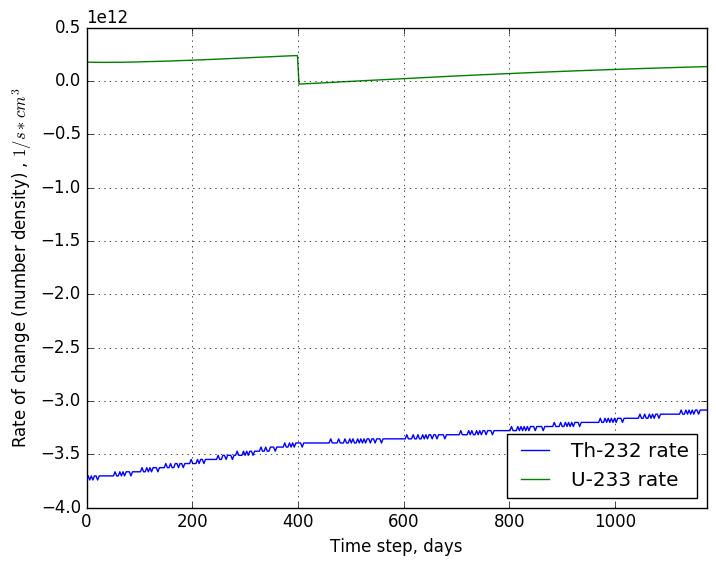
\includegraphics[height=0.75\textheight]{./images/rates_fuel.png}
   \vspace{-0.05in}
   \caption{Major isotopes rate of change during online reprocessing.}
    \end{figure}

    \column[t]{4.5cm}
       \begin{itemize}
        \item To keep the reactor critical, a higher $^{233}$U flow rate from the protactinium decay tank required for
the first 400 days.
   		\item The $^{232}$Th rate of loss slightly decreases over 4 years of operation due to fissile materials accumulation.
       \end{itemize}
     \end{columns}
\end{frame}

\begin{frame}
  \frametitle{Rate of change $^{233}$Pa, $^{233}$U from the protactinium decay tank}
    \begin{columns}
    \column[t]{8cm}
   \vspace{-0.35in}
  \begin{figure}[t]
   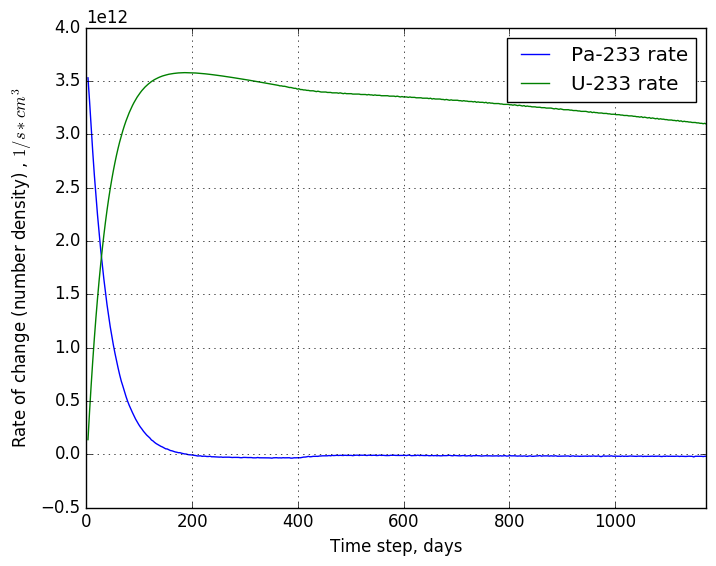
\includegraphics[height=0.8\textheight]{./images/rates_outflow.png}
   \vspace{-0.12in}
   \caption{Isotopes rate of change for the protactinium decay tank during MSBR online reprocessing.}
    \end{figure}

    \column[t]{4cm}
        \begin{itemize}
        \item Protactinium accumulated for approximately 200 days.
   		\item Fresh fissile $^{233}$U fuel flow established after 200 days.
   	  \end{itemize}
     \end{columns}
\end{frame}

\begin{frame}
  \frametitle{Neutron spectrum}
   \vspace{-0.5in}
  \begin{figure}[t]
   \hspace*{-0.39in}
   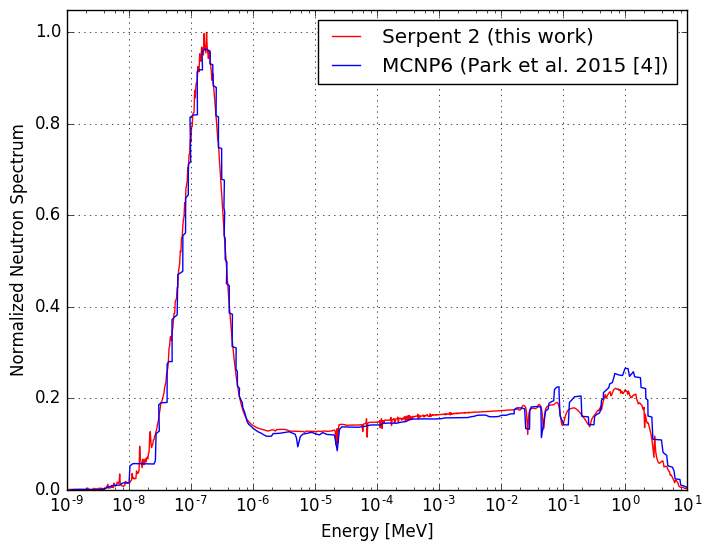
\includegraphics[height=0.8\textheight]{./images/spectrum.png}
   \vspace{-0.1in}
   \caption{Neutron spectrum for initial and equilibrium composition (normalized per lethargy).}
    \end{figure}
    \vspace{-0.1in}
    \begin{itemize}
       \item \gls{MSBR} has a epithermal spectrum which is perfect for thorium fuel cycle.
       \item Spectrum becames harder due to heavy fission products accumulation.
    \end{itemize}   
\end{frame}


\section{Conclusions}
\begin{frame}
  \frametitle{Conclusions}
        \begin{block}{This study outcomes}
        \begin{itemize}
                \item Full-core \gls{MSBR} 3-D analysis was performed using the SERPENT 2 Monte Carlo code.
                \item K$_{eff}$ for initial fuel composition is slightly larger than 1 (1.00397) which
                  allows reactor operation from startup to the first online reprocessing cycle.
                \item The neutron flux energy was calculated for the whole \gls{MSBR} core.
                \item The total temperature coefficient is negative, but MTC is negative which has a
                  negligible effect on safety because it is outweighed by the strong, negative FTC.
                \item Simulation results are in a good agreement with Park (MCNP6) model except moderator temperature
                  coefficient.
        \end{itemize}
        \end{block}
        
\end{frame}

\begin{frame}
  \frametitle{Conclusions}
         
              \begin{block}{Future research effort}
               This high-fidelity full-core model will be employed for:
               \begin{enumerate}
                \item Depletion simulations using SERPENT 2 capabilities to find the equliblium fuel composition of the \gls{MSBR}.
                \item Initial fuel salt composition and reprocessing parameters (i.e. rates of removing fission products,
                  the rate of refilling thorium) optimization.
                \item Problem-oriented nuclear data libraries generation for multi-physics models of \gls{MSBR} in the
                  MOOSE-based coupled neutronics/thermal-hydraulics code Moltres \cite{lindsay_arfc/moltres:_2017}.
               \end{enumerate}
               \end{block}
\end{frame}

%%--------------------------------%%
%%--------------------------------%%
\begin{frame}[allowframebreaks]
  \frametitle{References}
  \bibliographystyle{unsrt}
  {\footnotesize \bibliography{bibliography.bib} }

\end{frame}

%%--------------------------------%%
%%---BACKUP SLIDES----------------%%

\begin{frame}
  \frametitle{Generation IV Reactors}
              \begin{block}{Goals for Generation IV Nuclear Energy Systems \cite{ABRAM2008}}
               \begin{enumerate}
                \item Sustainability
                \item Economics
                \item Safety and Reliability
                \item Proliferation Resistance and Physical Protection
               \end{enumerate}
               \end{block}
               \begin{figure}[t]
                \vspace*{-0.1in}
                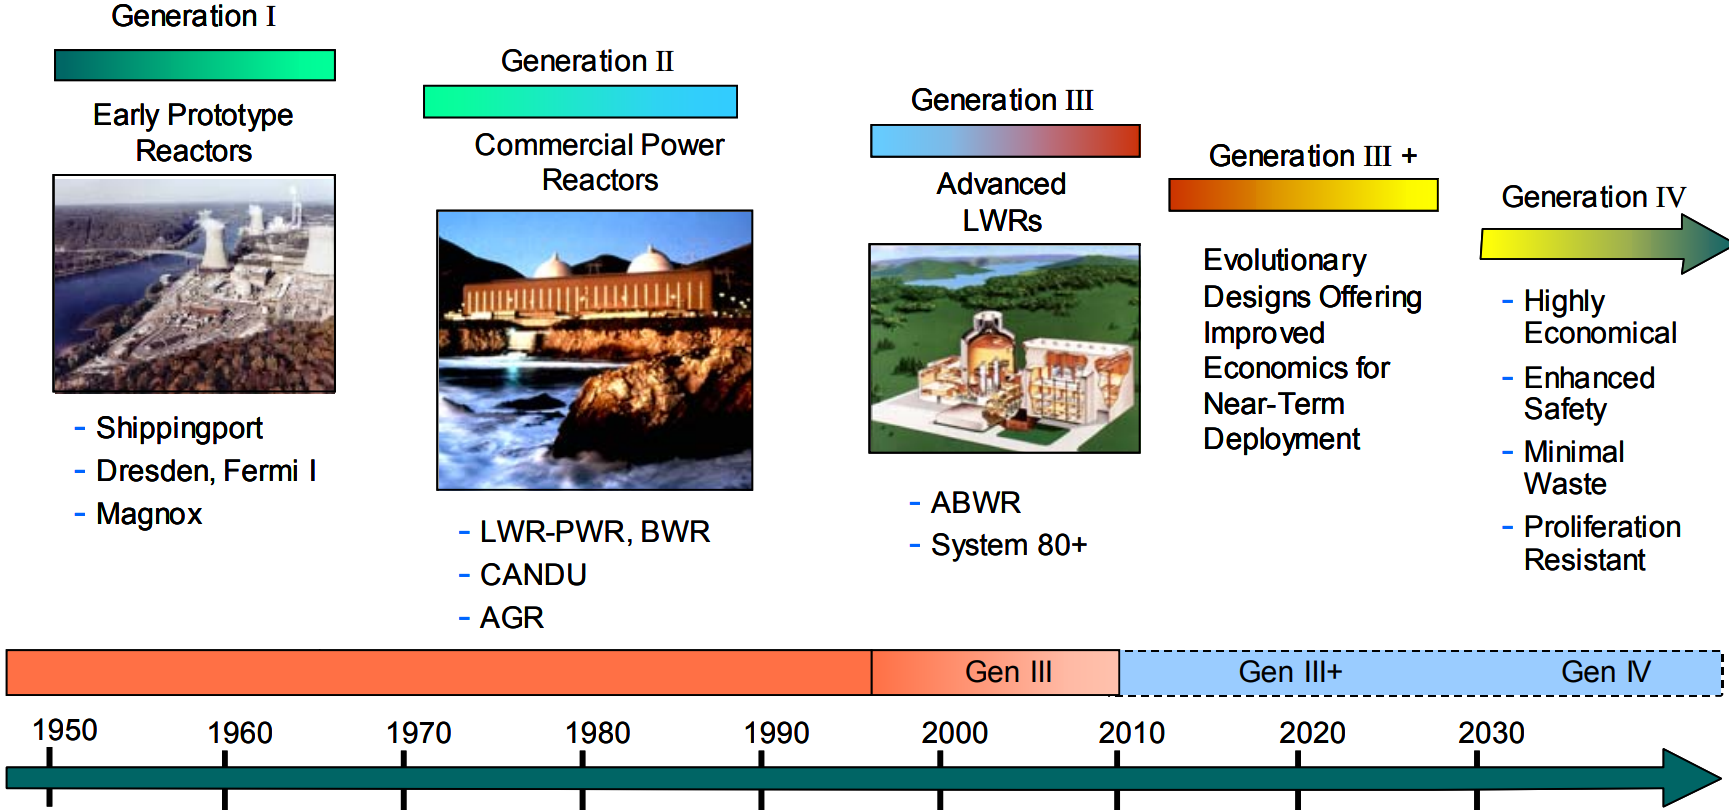
\includegraphics[height=0.4\textwidth]{./images/gen4_road_map.png}
                \vspace*{-0.1in}
                \caption{A Technology Roadmap for Gen IV Nuclear Energy Systems \cite{ABRAM2008}.}
               \end{figure}
              
\end{frame}

\end{document}



